\chapter{Projekt aplikacji}

\section{Architektura}

Architektura aplikacji jest złożona z części mobilnej oraz czterech serwisów, z czego każdy występuje jako autonomiczna aplikacja z którą porozumiewanie odbywa się za pomocą protokołu HTTP. Warstwa prezentacyjna, porozumiewając się z pozostałymi serwisami zapewnia użytkownikowi płynną interakcję z systemem w celu osiągnięcia zamierzonych akcji dostępnych w obrębie funkcjonalności.\\
W ten sposób każda składowa część aplikacji może być niezależnie zarządzana. W momencie w którym pojedynczy element odpowiedzialny za szczególną usługę jest wyłączony, sama aplikacja może dalej działać wyłączając tylko funkcjonalności dostarczane przez niedostępny aktualnie serwis.\\
\linebreak
Takie podejście można określić mianem zorientowanym na usługi. Oznacza to, że przy tworzeniu systemu, spory nacisk kładziony jest na definiowanie spełniających wymagania użytkownika usług. Są one elementami oprogramowania zdolnymi do niezależnego funkcjonowania, udostępniającymi realizowane funkcje poprzez zdefiniowany interfejs.\\
\linebreak
HTTP (\texttt{Hypertext Transfer Protocol}), czyli "Protokół Przesyłania Danych Hipertekstowych to protokół warstwy aplikacji, odpowiedzialny za transmisję dokumentów hipermedialnych, jak np. HTML. Został stworzony do komunikacji pomiędzy przeglądarkami, a serwerami webowymi, ale może być używany również w innych celach. HTTP opiera się na klasycznym modelu klient-serwer, gdzie klient inicjuje połączenie poprzez wysłanie żądania, następnie czeka na odpowiedź. HTTP jest protokołem bezstanowym, co oznacza, że serwer nie przechowuje żadnych danych (stanów) pomiędzy oboma żądaniami. (...) "~\cite{http}
\linebreak

\begin{figure}[H]
	\centering
	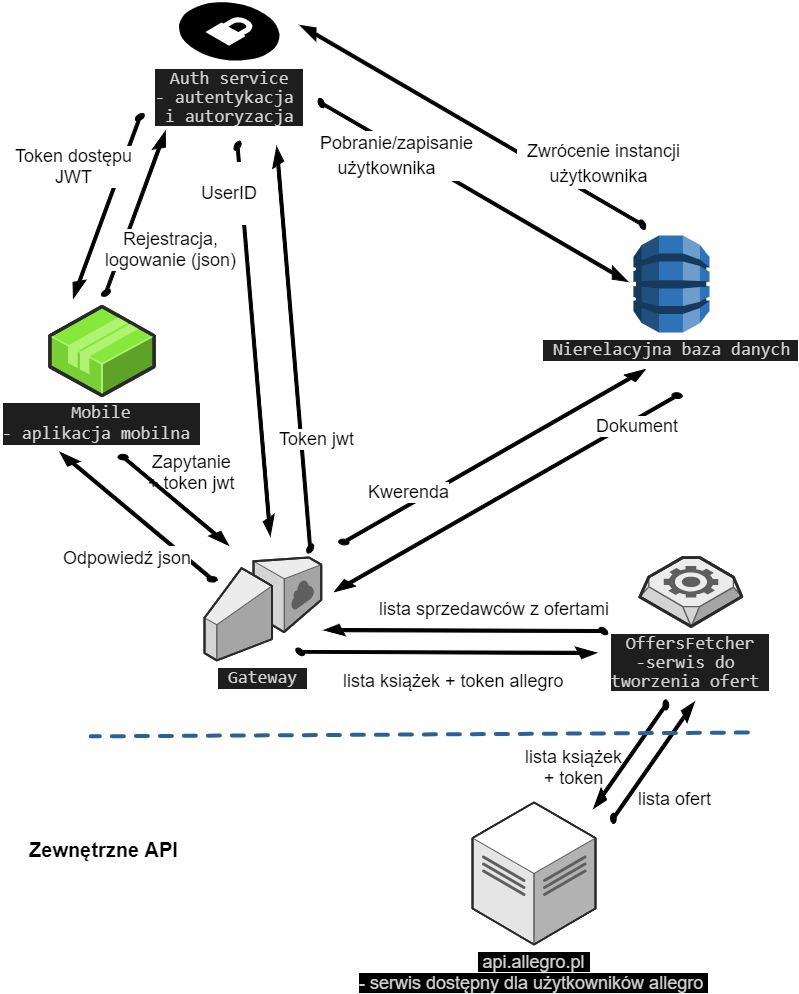
\includegraphics[width=\linewidth]{architecture_overview.png}
	\caption{Rysunek poglądowy struktury}
\end{figure}

\section{Auth service}
Auth service dba o zachowanie bezpieczeństwa w całym systemie.
Poprzez ekstrakcję funkcjonalności związanej z tworzeniem kont, logowaniem oraz zarządzaniem dostępem do pozostałych sektorów, gwarantuje niezawodną autentykację i autoryzację użytkownika pragnącego korzystać z aplikacji.\\
Informacje o kontach użytkowników przechowywane są w bazie danych, do której dostęp uzyskać można tylko za pomocą wygenerowanego przez nią, wewnętrznego klucza. 
\\
W celu swobodnego poruszania się po aplikacji należy uzyskać JWT(\texttt{JSON Web Token}). Aby pozsykać token należy się zarejestrować lub zalogować na ekranie logowania. Zapytanie utworzone w ten sposób zostanie wysłane do Auth service. W odpowiedzi przesłany zostanie wyżej wymieniony klucz dostępowy.\\

\subsection{JSON Web Token}

JSON Web Token to otwarty standard, który definiuje kompaktowy i samodzielny sposób na bezpieczny transfer danych. Poszczególna instancja składa się z trzech części oddzielonych kropkami w bezpośrednim formacie xx..x.y..yy.zz..z, gdzie poszczególne człony reprezentują: \cite{jwt}
\begin{enumerate}%[1)]
	\item Header - nagłówek, zawierający dwie informacje:
		\begin{itemize}
			\item typ tokenu, w tym przypadku "JWT"
			\item algorytm szyfrujący(n.p. HMAC, SHA256 lub RSA)
		\end{itemize}

	\item Payload - lista wyrażeń opisujących szyfrowaną informację, w przypadku użytkownika - np jego login, czy email.
	
	\item Signature - podpis stworzony poprzez zaszyfrowanie podanym w headerze algorytmem szyfrującym ciągu składającego się z
	\begin{itemize}
		\item zakodowanego za pomocą Base64 (specjalnego kodowania transportowego) nagłówka i listy wyrażeń
		\item sekretu, czyli unikalnego dla danych klucza.
	\end{itemize}
	\end{enumerate}

	\begin{figure}[H]
		\centering
		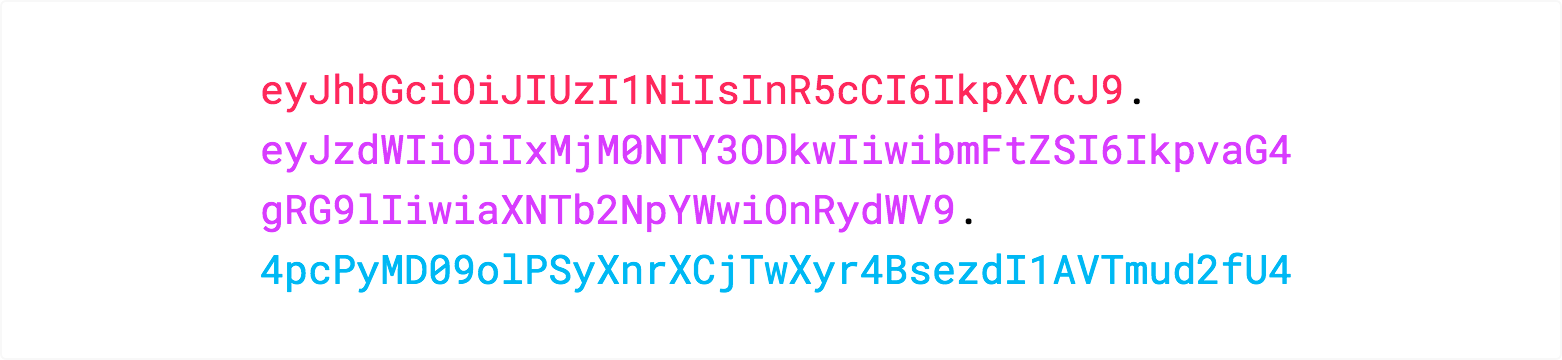
\includegraphics[width=\linewidth]{json-token.png}
		\caption{Przykładowy token jwt \cite{jwt}}
	\end{figure}

\subsection{JSON Web Token}


\section{Gateway}
\section{Obliczanie ofert}
\section{Baza danych}
\section{Aplikacja mobilna}
\section{Zewnętrzne API}